\begin{frame}{Mutation}
    \begin{columns}[T] % T aligns the tops of the columns
        \begin{column}{0.75\textwidth}
            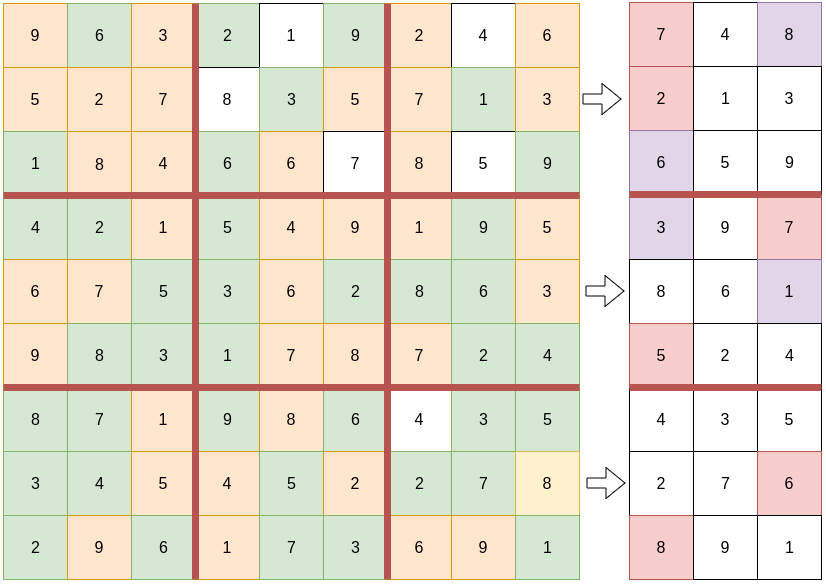
\includegraphics[width=\textwidth]{Pictures/Mutation.png}
        \end{column}
        \begin{column}{0.35\textwidth}
            \begin{itemize}
                \item Ausführung blockweise
                \item gegebene Felder werden ignoriert
            \end{itemize}
            \begin{enumerate}
                \item Auswählen von Kollisionszellen (beliebige Chance für andere Zellen) 
                \item zufälliges paarweises Austauschen der gewählten Zellen
            \end{enumerate}
        \end{column}
    \end{columns}
    \note[item]{grid-repraesentation und Fitness-Sudoku benoetigt}
    \note[item]{blockweise ausgefuehrt}
    \note[item]{gruen bleibt, rot tauschen, weiss Wahrscheinlichkeits tausch}
    \note[item]{--> Feld mit 1 Kollision kann trotzdem noch tauschen}
    \note[item]{weniger Minima -> groessere Exploration}
    \note[item]{Liste aller Zahlen}
    \note[item]{Zufaelliges Auswaehlen von Tauschpaaren}
    \note[item]{uebrige zurueckschreiben}
\end{frame}
